\chapter{Calendrier et répartition des tâches}

%============= Calendrier ===================
\section{Calendrier}

% Nous avons choisi de fonctionner ainsi, car la contrainte de créneaux n'est pas propice à la motivation. D'un point de vue global, le temps alloué au PAO correspondra bien au temps semestriel de 3 crédits ECTS chacun, soit 180 heures à nous deux.\\

% ============= Répartition des tâches ===================
\section{Répartition des tâches}
La répartition des tâches s'est découpée comme présentée sur la figure suivante.


% \begin{figure}
% \hspace{-1cm}
% \begin{tabular}{|@{}l@{}l}
% 	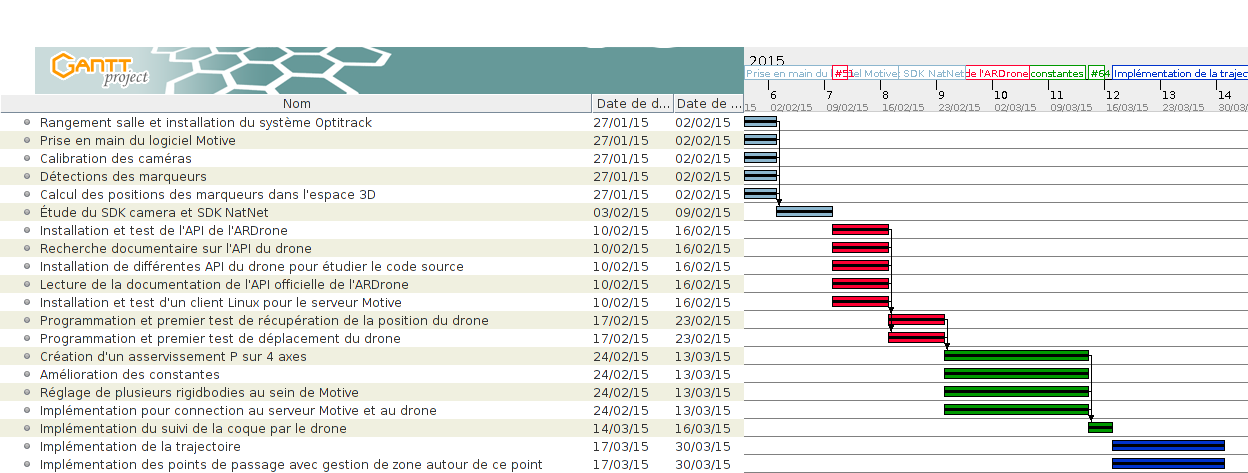
\includegraphics[width=24cm,angle=90]{images/calendrier.png}
% &
% 	\includegraphics[width=24cm,angle=90]{images/repartitionCharge.png}
%  \end{tabular}
%  \caption{Rétro-calendrier et Répartition des tâches}
%  \end{figure}
